%%%%%%%%%%%%%%%%%%%%%%%%%%%%%%%%%%%%%%%%%%%%%%%%%%%%%%%%%%%%%%%%%%%%%%%%
%    INSTITUTE OF PHYSICS PUBLISHING                                   %
%                                                                      %
%   `Preparing an article for publication in an Institute of Physics   %
%    Publishing journal using LaTeX'                                   %
%                                                                      %
%    LaTeX source code `ioplau2e.tex' used to generate `author         %
%    guidelines', the documentation explaining and demonstrating use   %
%    of the Institute of Physics Publishing LaTeX preprint files       %
%    `iopart.cls, iopart12.clo and iopart10.clo'.                      %
%                                                                      %
%    `ioplau2e.tex' itself uses LaTeX with `iopart.cls'                %
%                                                                      %
%%%%%%%%%%%%%%%%%%%%%%%%%%%%%%%%%%
%
%
% First we have a character check
%
% ! exclamation mark    " double quote  
% # hash                ` opening quote (grave)
% & ampersand           ' closing quote (acute)
% $ dollar              % percent       
% ( open parenthesis    ) close paren.  
% - hyphen              = equals sign
% | vertical bar        ~ tilde         
% @ at sign             _ underscore
% { open curly brace    } close curly   
% [ open square         ] close square bracket
% + plus sign           ; semi-colon    
% * asterisk            : colon
% < open angle bracket  > close angle   
% , comma               . full stop
% ? question mark       / forward slash 
% \ backslash           ^ circumflex
%
% ABCDEFGHIJKLMNOPQRSTUVWXYZ 
% abcdefghijklmnopqrstuvwxyz 
% 1234567890
%
%%%%%%%%%%%%%%%%%%%%%%%%%%%%%%%%%%%%%%%%%%%%%%%%%%%%%%%%%%%%%%%%%%%
%
\documentclass[12pt]{iopart}
\newcommand{\gguide}{{\it Preparing graphics for IOP Publishing journals}}
%Uncomment next line if AMS fonts required
%\usepackage{iopams}  
\usepackage{graphicx} 
\usepackage{xcolor}

\begin{document}

\title[]{Identification of  nuclear recoils in gas  with a sCMOS camera}

\author{A Marco Emanuele, Cavoto Gianluca, Pinci Davide}

\address{San Miguel, Mexico}
\ead{emanuele.a.marco@roma1.infn.it}
\vspace{10pt}
\begin{indented}
\item[]May 2020
\end{indented}

\begin{abstract}

\end{abstract}

%
% Uncomment for keywords
%\vspace{2pc}
%\noindent{\it Keywords}: XXXXXX, YYYYYYYY, ZZZZZZZZZ
%
% Uncomment for Submitted to journal title message
%\submitto{\JPA}
%
% Uncomment if a separate title page is required
%\maketitle
% 
% For two-column output uncomment the next line and choose [10pt] rather than [12pt] in the \documentclass declaration
%\ioptwocol
%



\section{Introduction}

The advent of a market of high position resolution and single photon  light sensors can open new opportunity to investigate ultra-low rate phenomena as Dark Matter  (DM) particle  scattering on nuclei in a gaseous  target.

The nature of DM is still one of the key  issues to understand  our Universe. Different models  predicts the existence of neutral particles with a mass of GeV  or higher that would fill our Galaxy. They  could interact with the nuclei present in ordinary matter producing highly ionizing nuclear recoils but with a  kinetic energy as small as  few keV. Moreover, given the motion of the Sun in the Milky Way towards the Cygnus constellation such nuclear recoils would exhibit a dipole angular distribution in a terrestrial detector.
In this paper we describe the use of a scientific CMOS camera to capture the light emitted by Gas Electron Multipliers (GEMs) in a Time Projection Chamber (TPC) device. The GEMs are located in the TPC gas volume at the anode position and are used to convert the ionization produced in the gas by   the  nuclear recoils into flashes of visible light. The flash of light can be located in space and its shape adopting a cluster  recognition algorithm.
 
 
 \section{Experimental layout and data }
 
 \section{Cluster pattern recognition}
 
 \section{Cluster observables}
 
 \section{Nuclear recoil identification results}
 
 \section{Conclusion and Outlook}
 
 
\begin{figure}[ht]
	\centering
	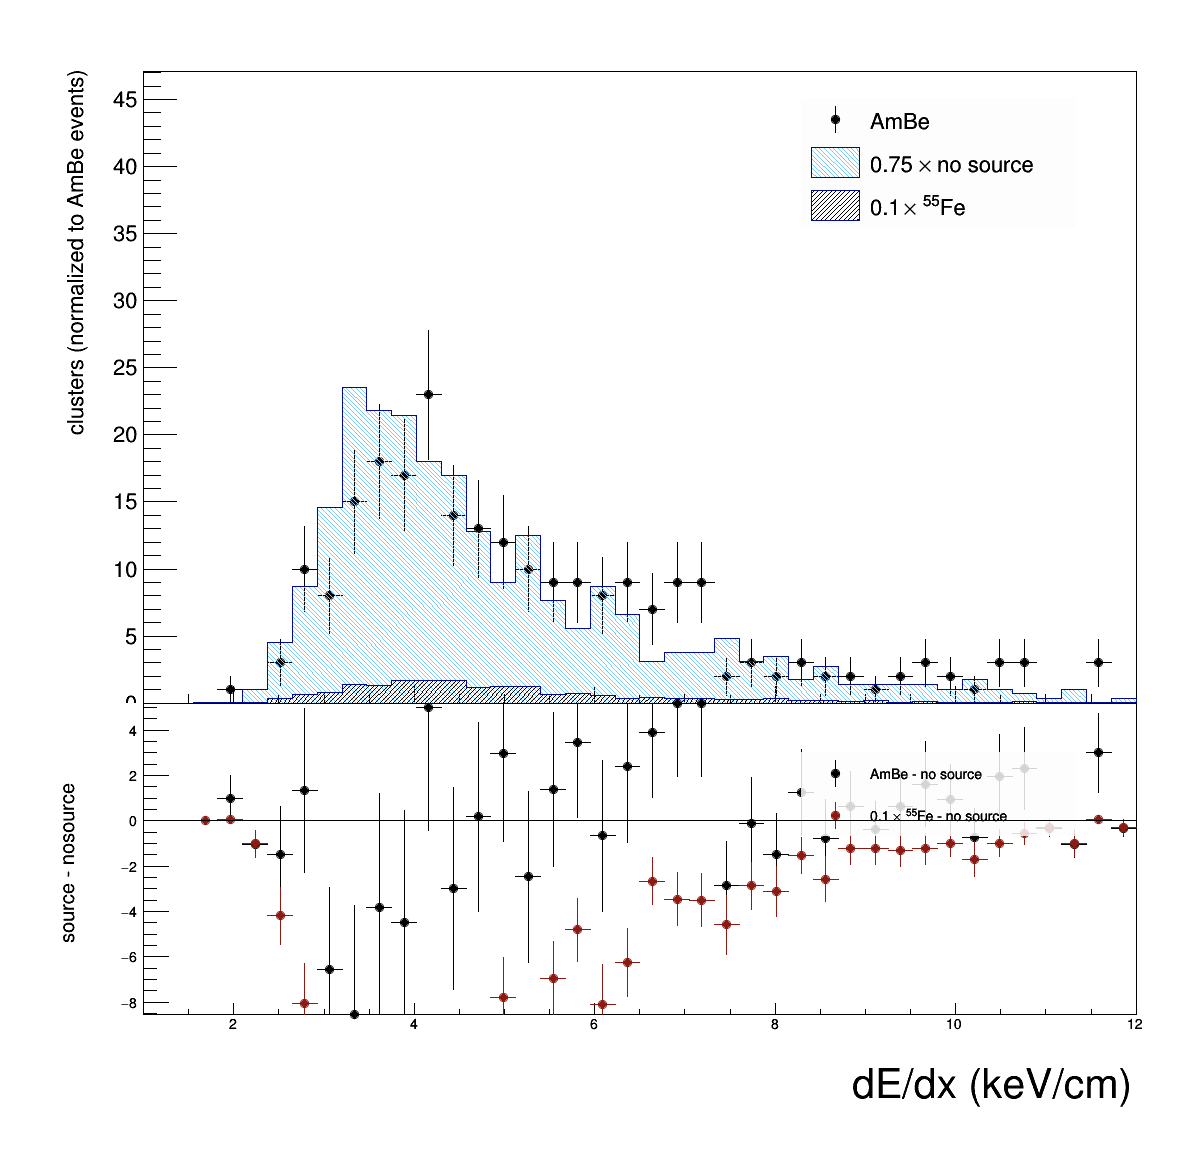
\includegraphics[width=0.45\linewidth]{dEdx_cosmics.png}
	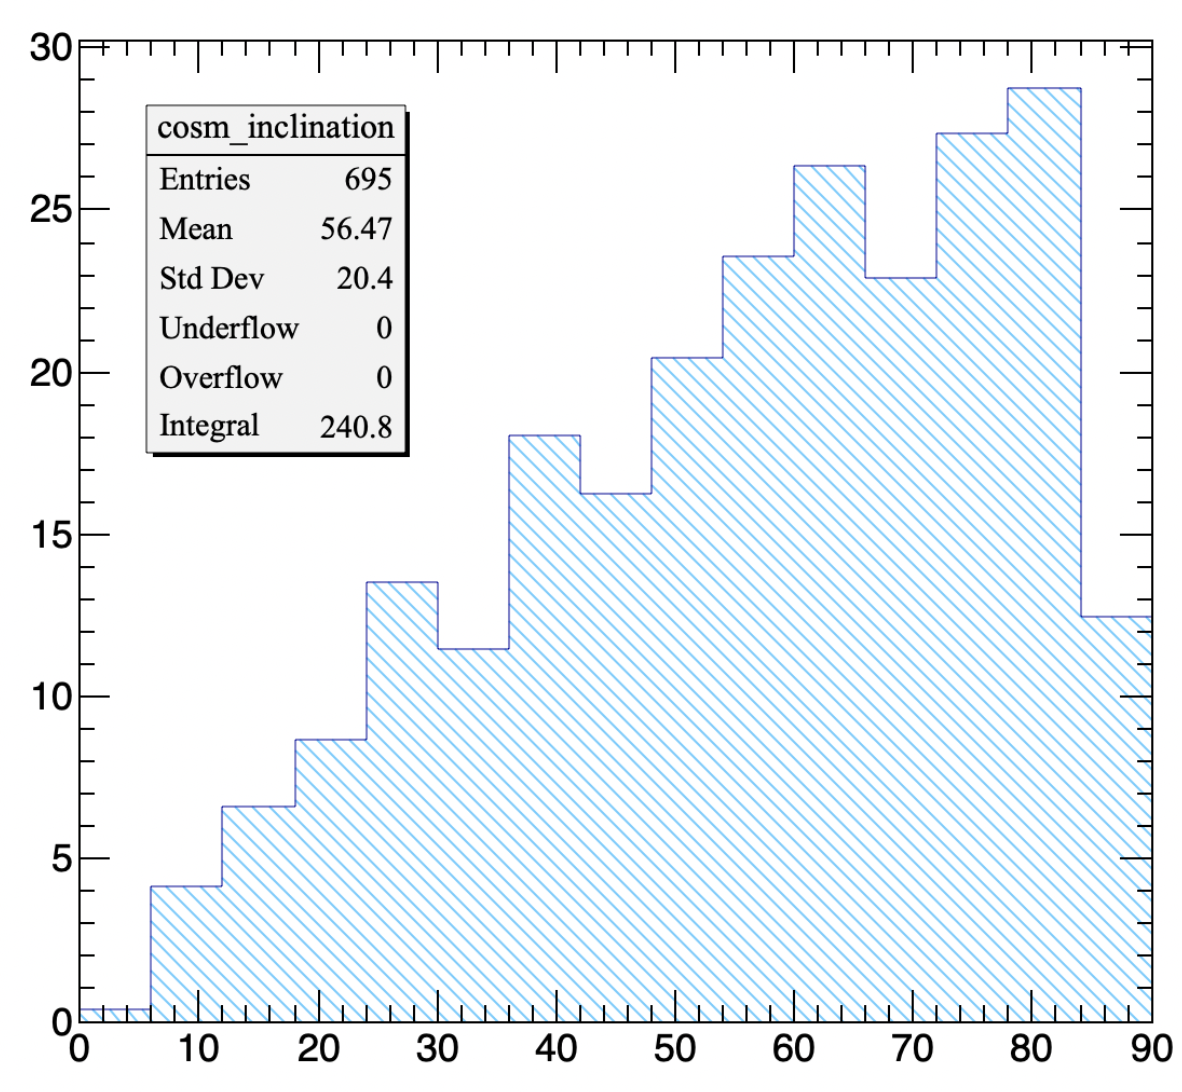
\includegraphics[width=0.45\linewidth]{cosmic_angle.png}
  	\caption{Left: Distributions of reconstructed angles for cosmic rays. Right: Distributions of reconstructed energy release per centimetre for cosmic rays.}
  	\label{fig:cosmics}
\end{figure}
\textcolor{red}{Non farei vedere il Ferro in questa figura. Inoltre il plot delle differenza deve essere fatto su scala diversa. }


\begin{figure}[ht]
	\centering
	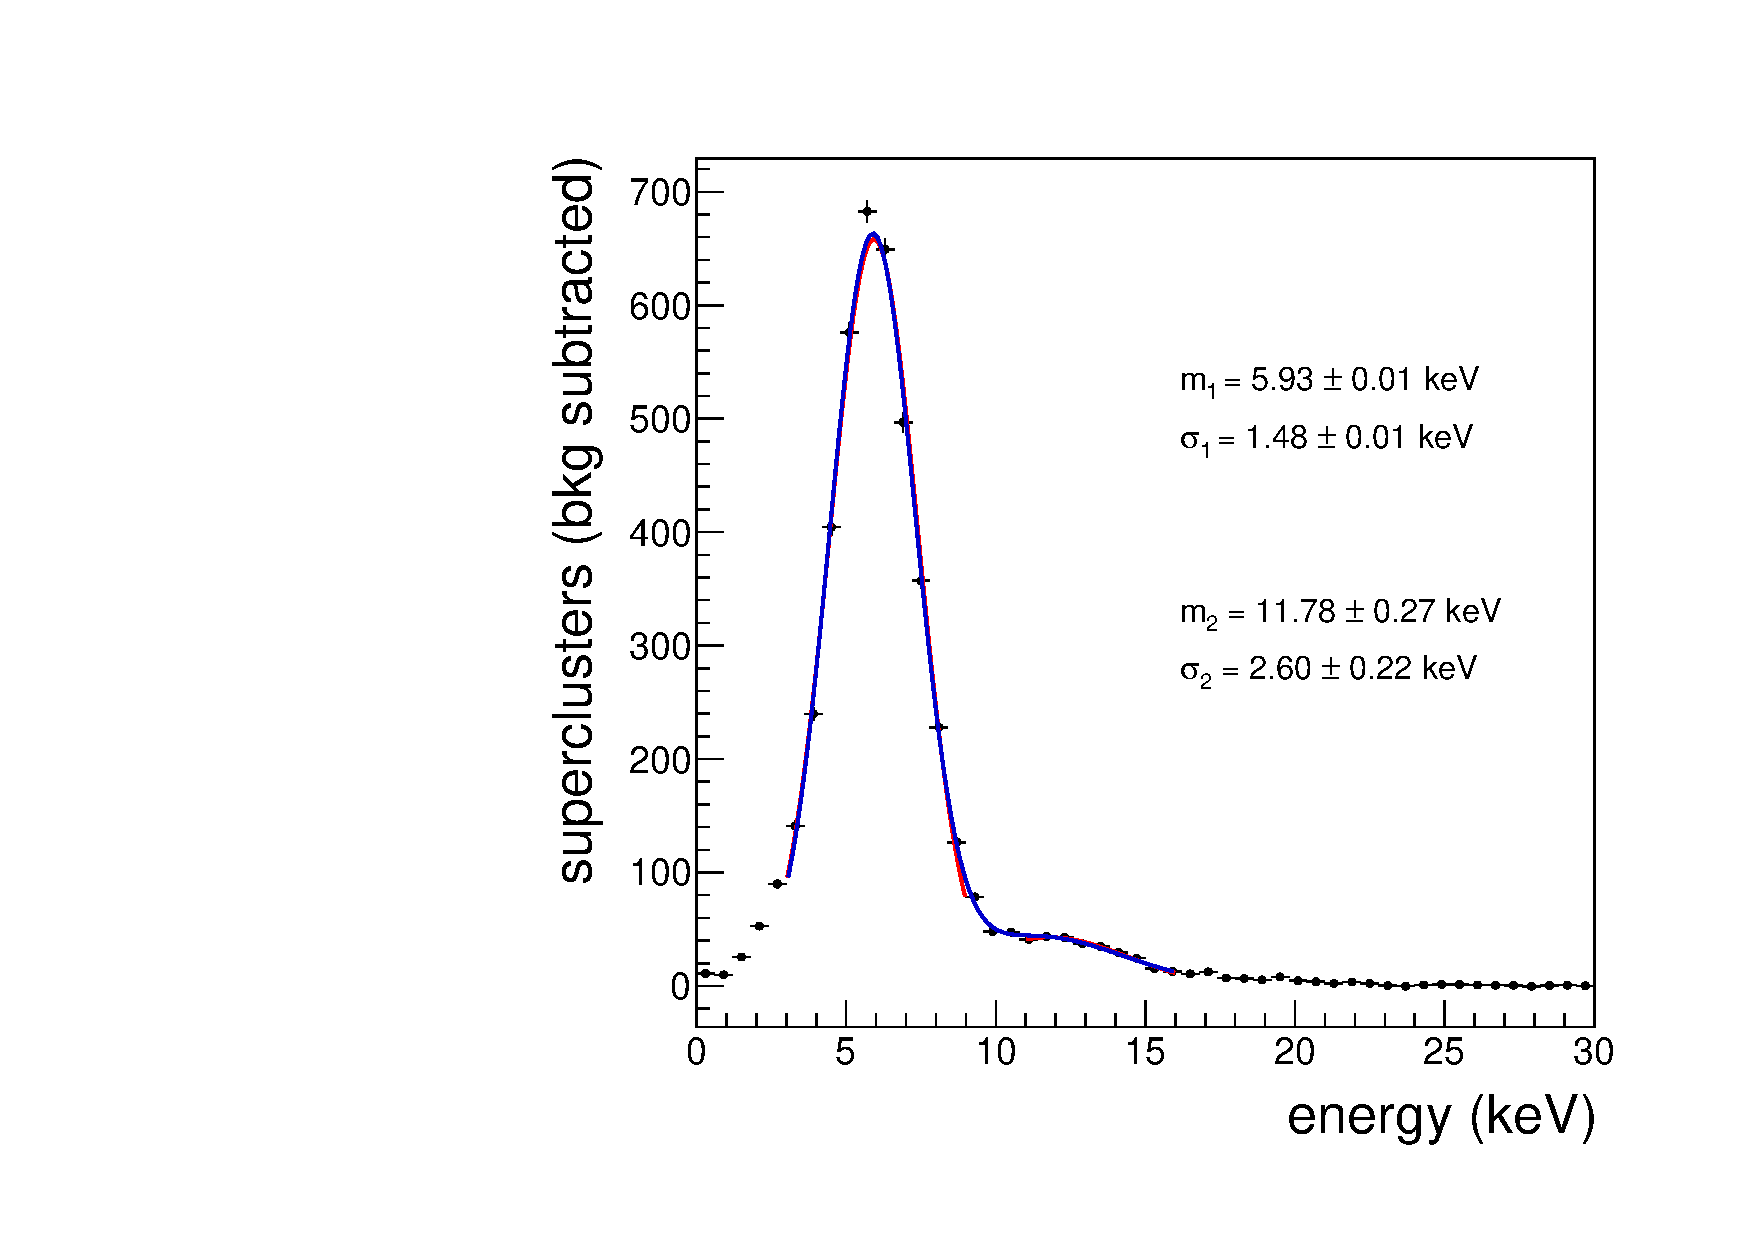
\includegraphics[width=0.45\linewidth]{fe_diff_simplefit.pdf}
	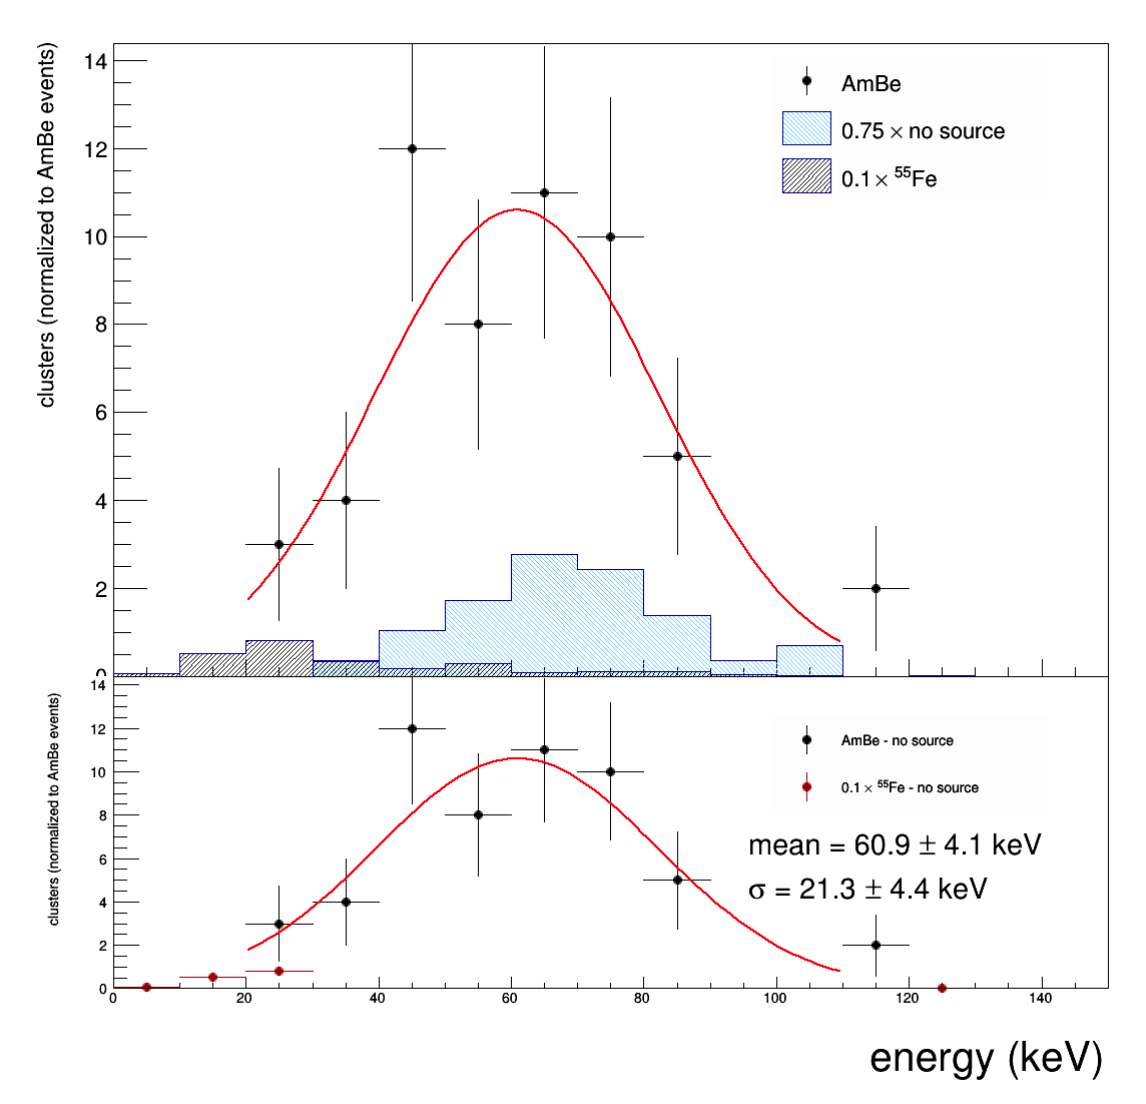
\includegraphics[width=0.45\linewidth]{spectrum_59keV.png}
  	\caption{Left: Spectrum of energy of the clusters reconstructed as produced by interactions of 5.9~keV photons in gas. Right: Spectrum of energy of the clusters reconstructed as produced by interactions of 59~keV photons in gas.}
  	\label{fig:55Fe&59keV}
\end{figure}

\begin{figure}[ht]
	\centering
	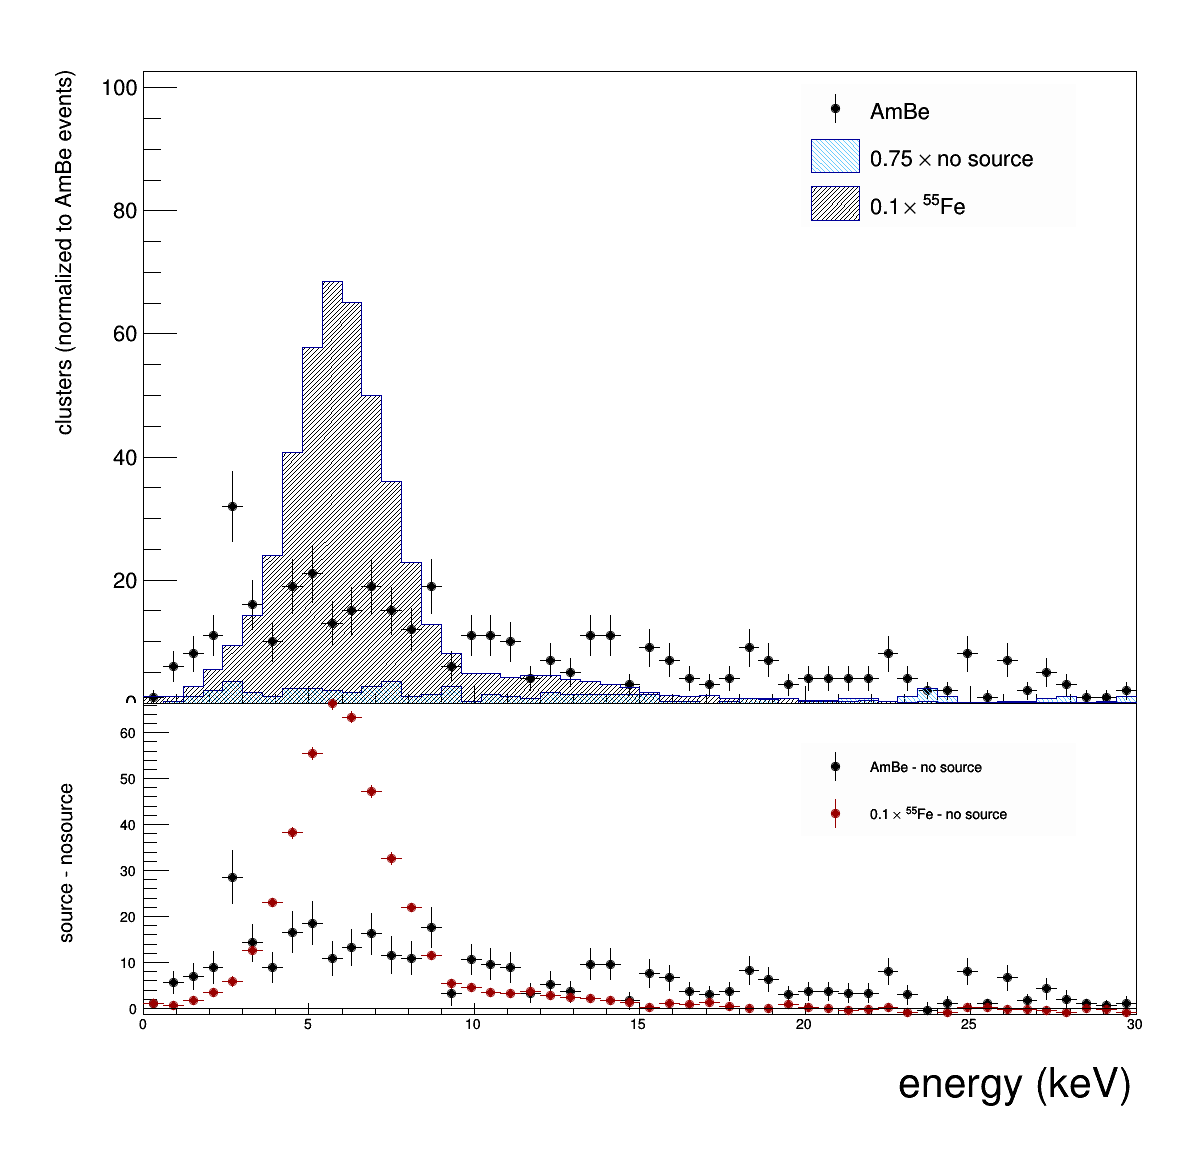
\includegraphics[width=0.45\linewidth]{energy_spectrum.png}
	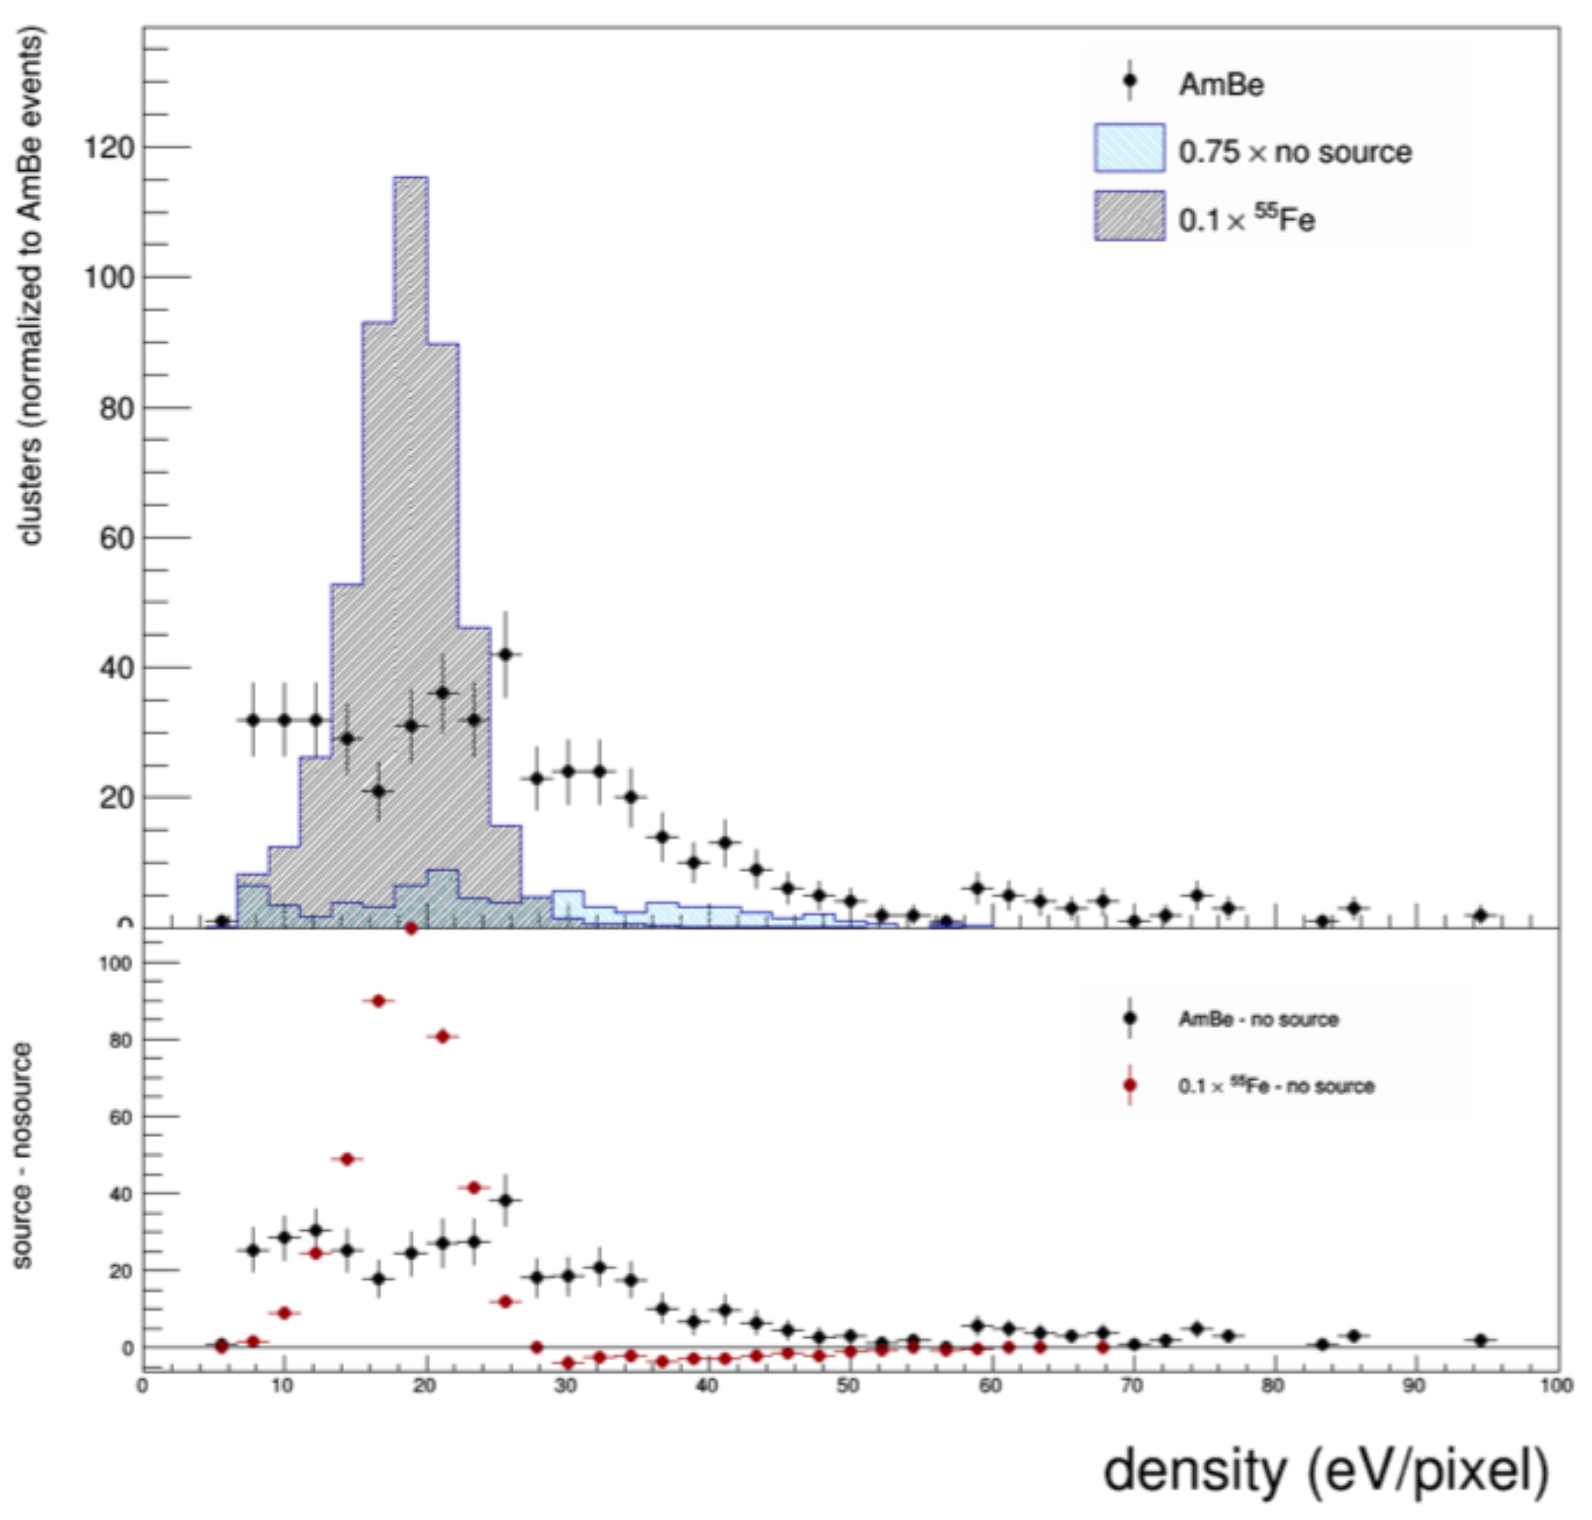
\includegraphics[width=0.45\linewidth]{density_spectrum.png}
  	\caption{Spectra of energy (left) and energy density (right) of the clusters reconstructed in three different run types after the preliminary cuts.}
  	\label{fig:ene&dens}
\end{figure}

\begin{figure}[ht]
	\centering
	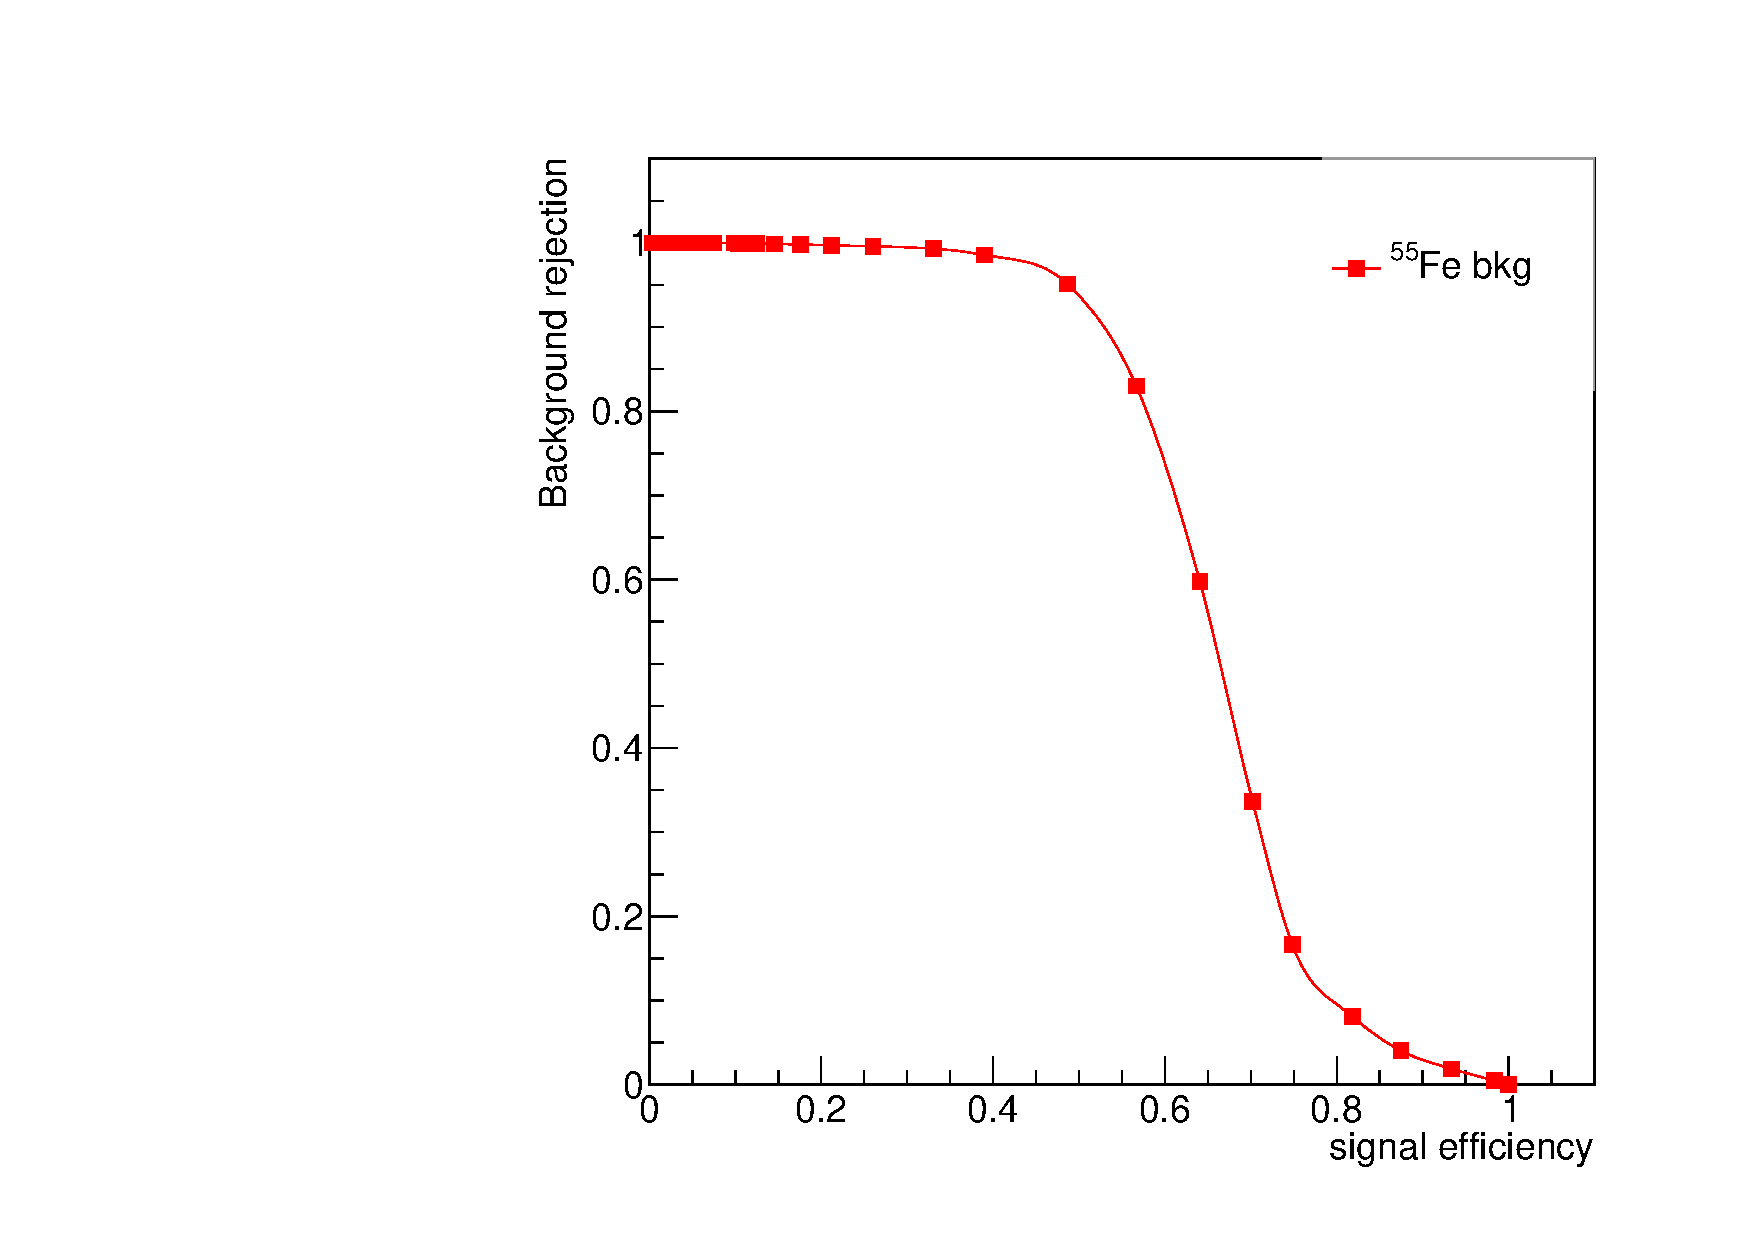
\includegraphics[width=0.50\linewidth]{density_roc.pdf}
  	\caption{Electron Recoil (ER) signal rejection as a function of the Nuclear Recoil signal detection efficiency.}
  	\label{fig:roc}
\end{figure}
\textcolor{red}{per un paio di punti scriverei vicino il taglio density > ...}

\begin{figure}[ht]
	\centering
	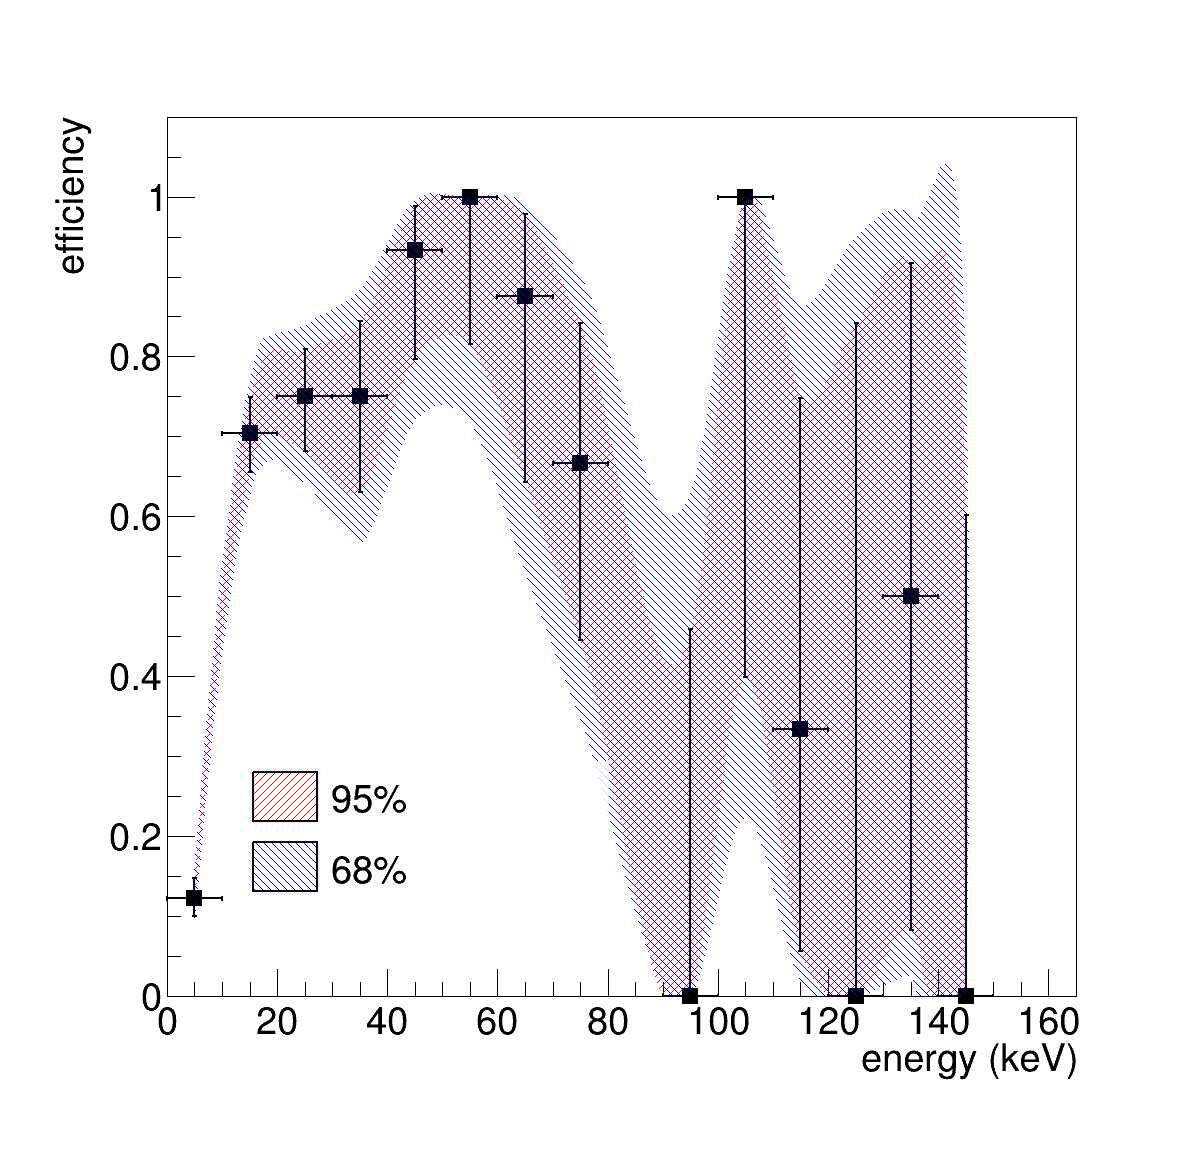
\includegraphics[width=0.45\linewidth]{effS.png}	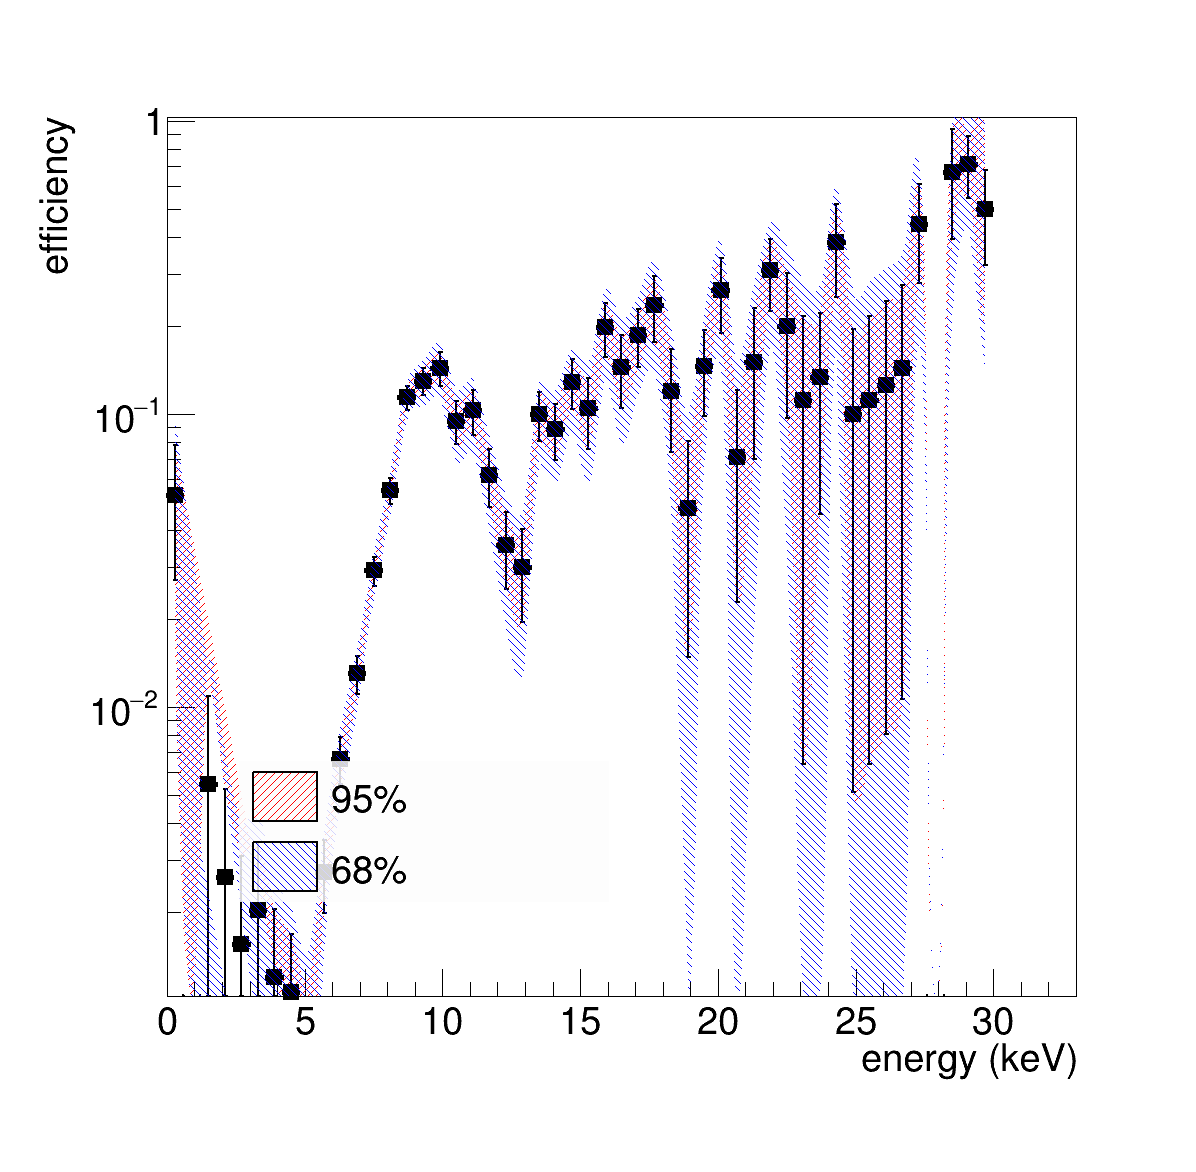
\includegraphics[width=0.45\linewidth]{effB.png}
  	\caption{Detection efficiency of Nuclear Recoil (NR) signals (left) and Electron Recoil (ER) signals (right) as a function of their reconstructed energy.}
  	\label{fig:effB}
\end{figure}


\begin{figure}[ht]
	\centering
	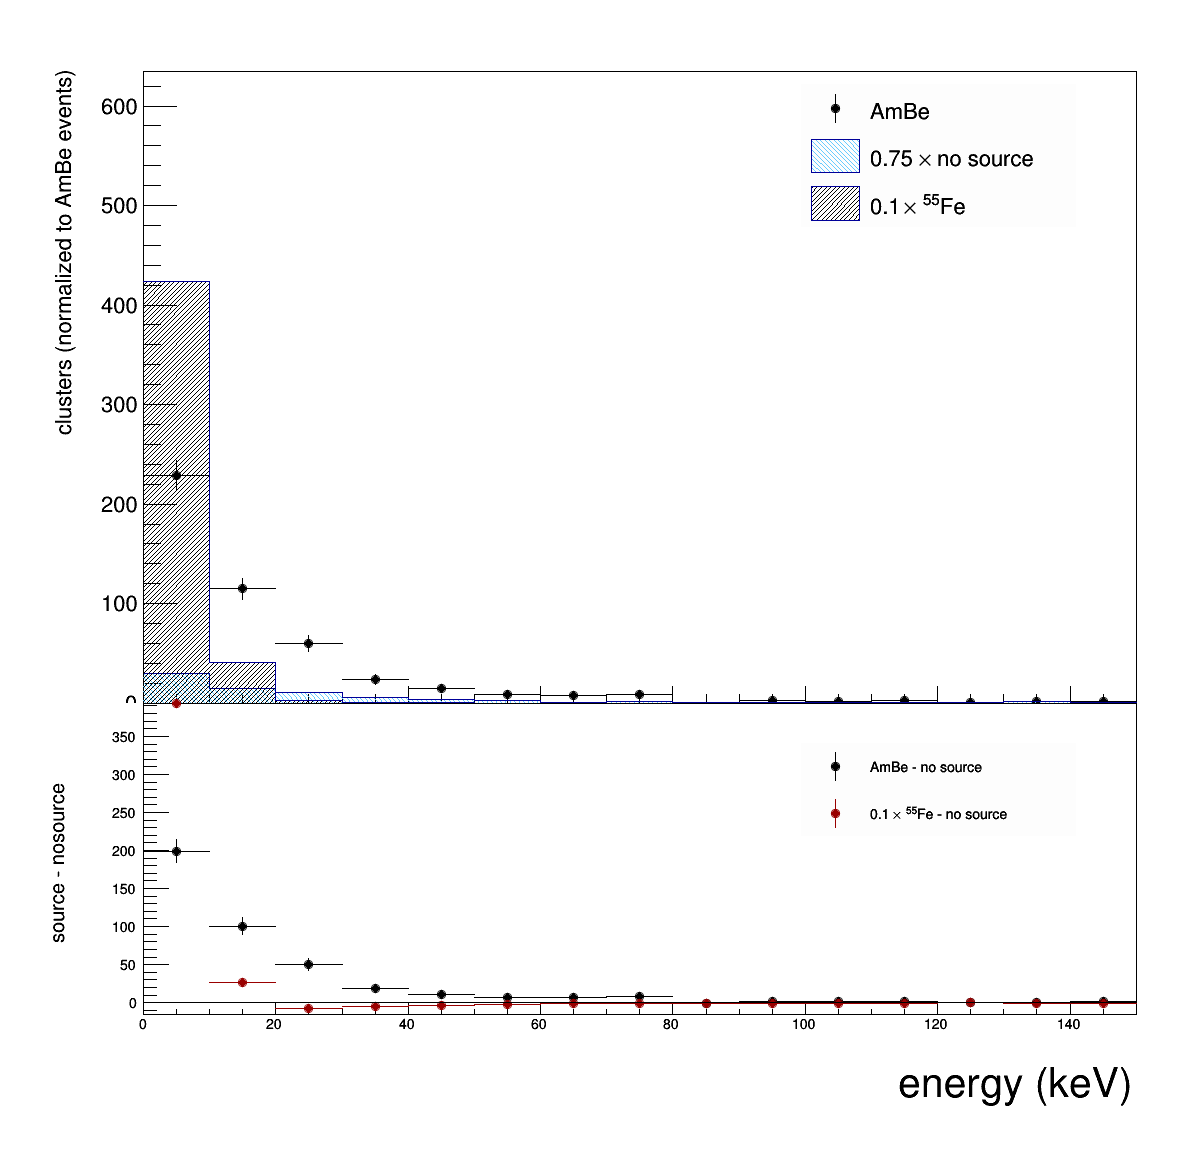
\includegraphics[width=0.45\linewidth]{energyExt.png}
	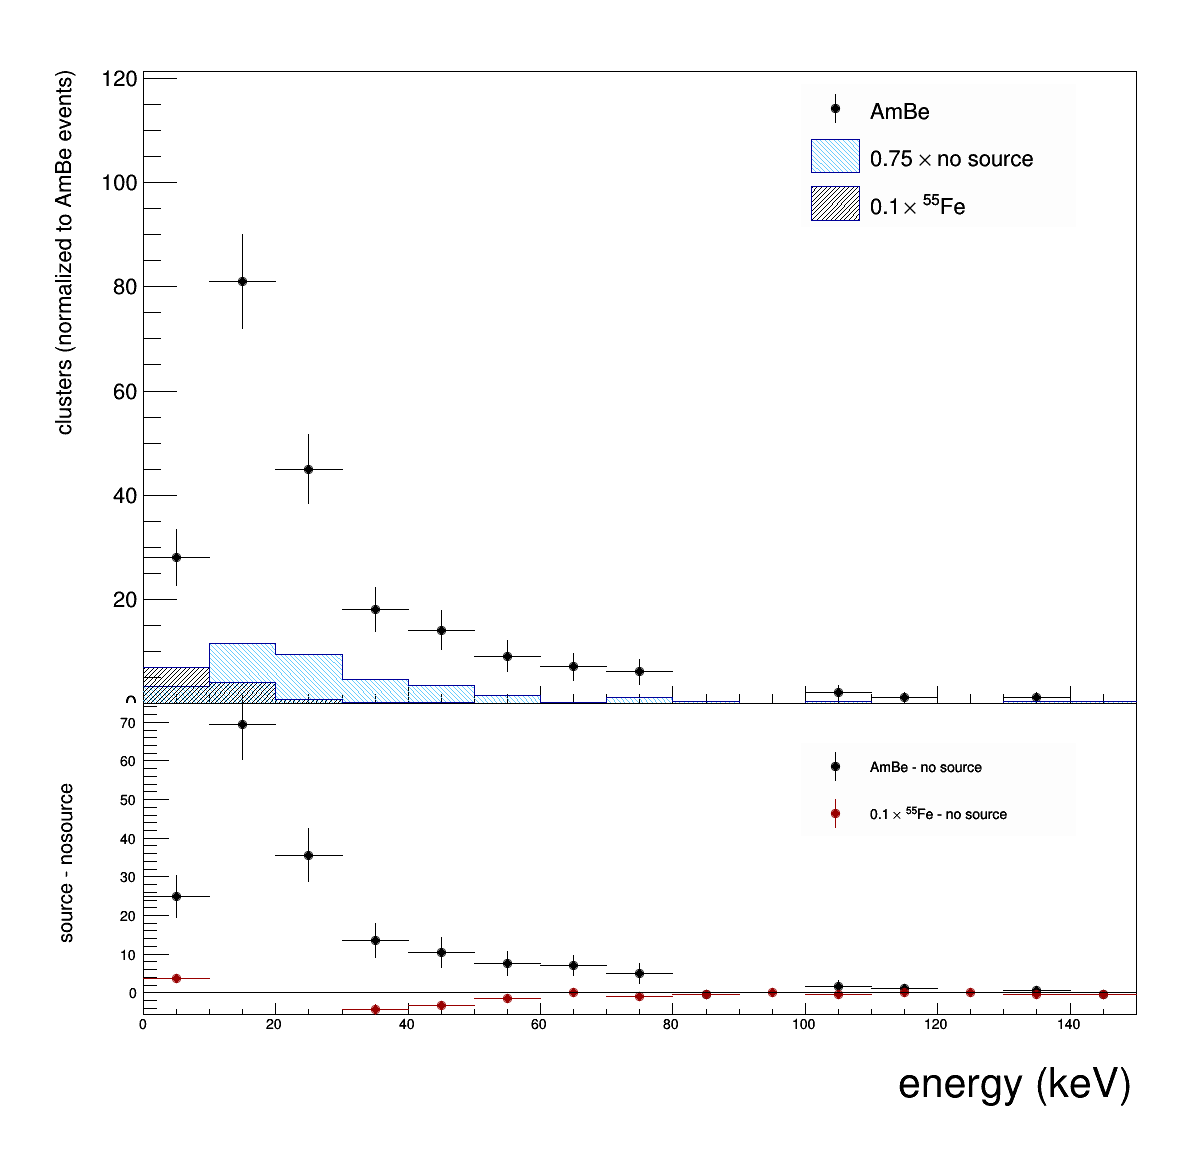
\includegraphics[width=0.45\linewidth]{energyExt_cut.png}
  	\caption{Spectra of energy of the clusters reconstructed in three different run types before (left) and after (right) cuts on energy densities.}
  	\label{fig:energy}
\end{figure}

\begin{figure}[ht]
	\centering
	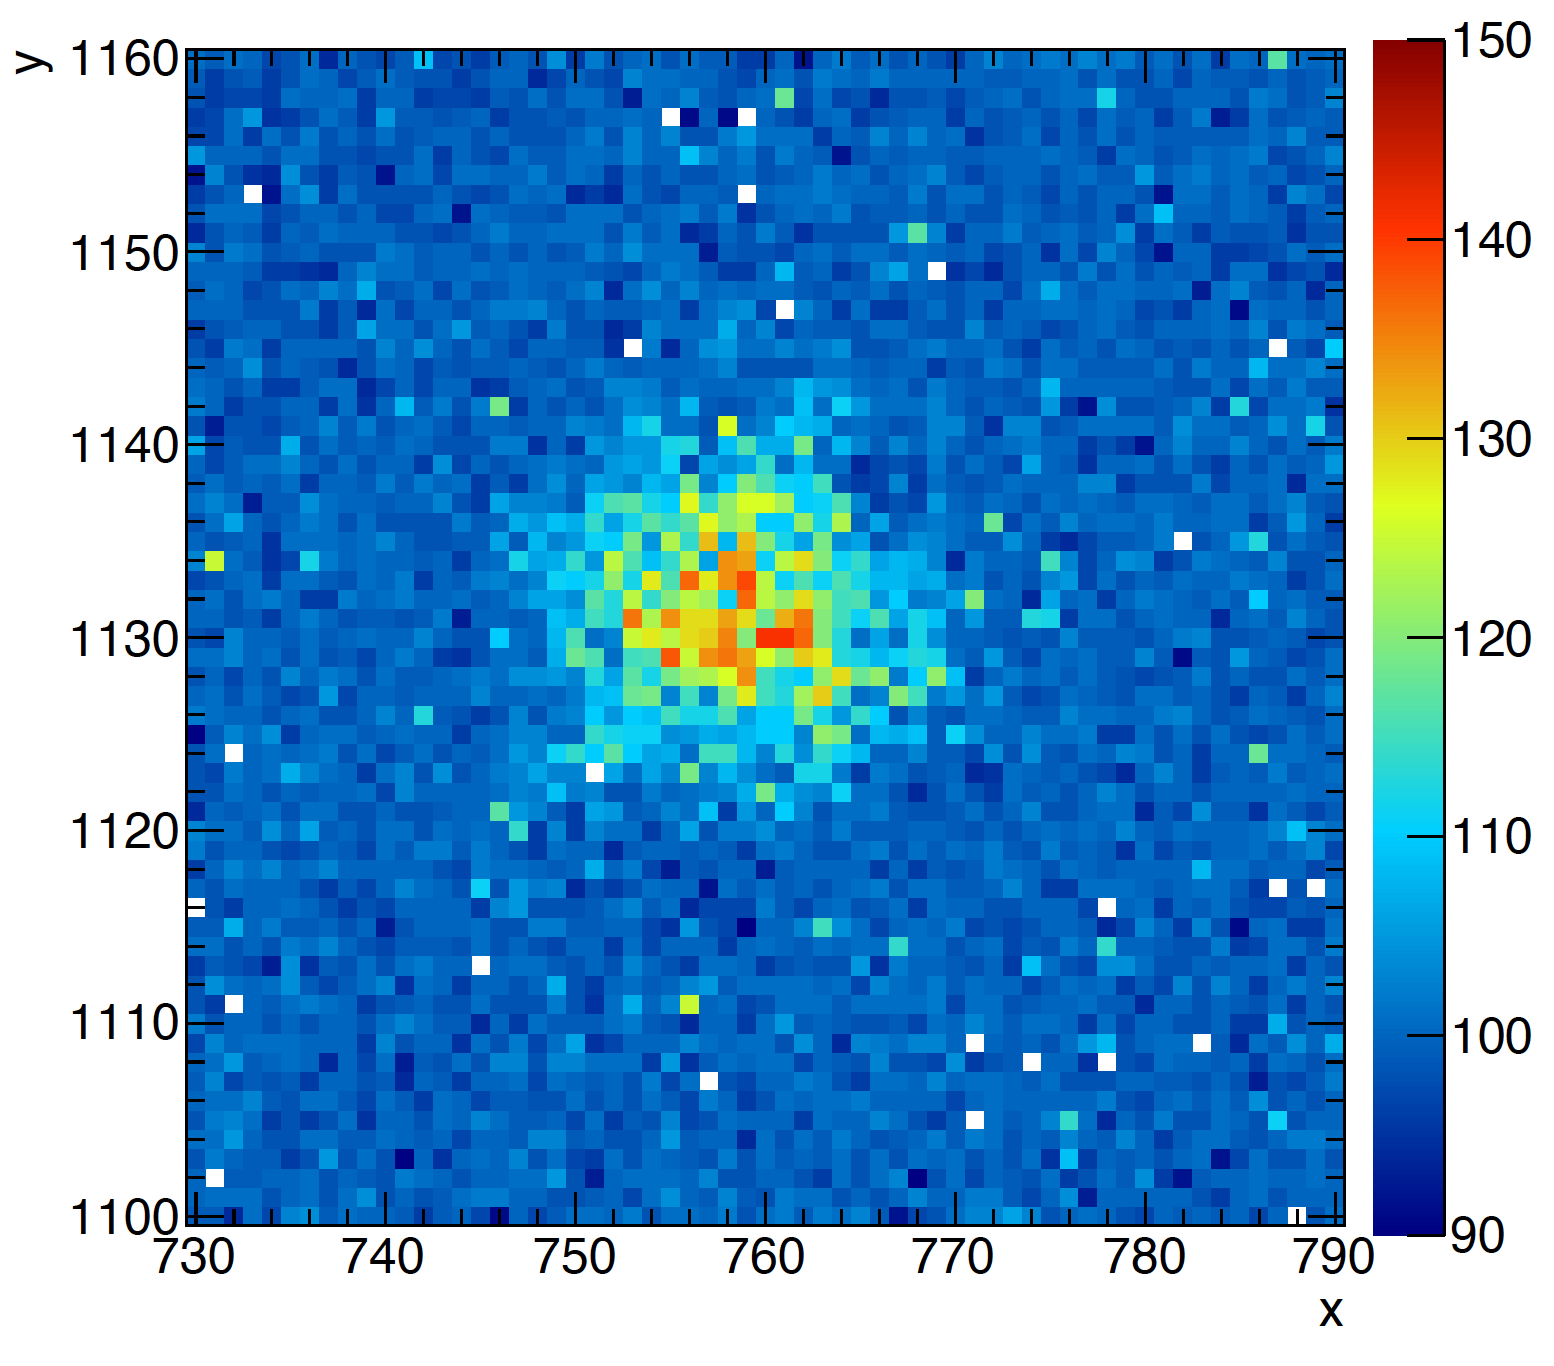
\includegraphics[width=0.50\linewidth]{granchio.png}
  	\caption{Example of a signal reconstructed as a Nuclear Recoil (NR) with an energy of 9~keV.}
  	\label{fig:granchio}
\end{figure}

\textcolor{red}{non farei vedere electron recoil che non ha senso in funzione dell'energia con questo campione }


\bibliography{mybiblio}

\end{document}

